%%%%%%%%%%%%%%%%%%%%%%%%%%%%%%%%%%%%%%%%%%%%%%%%%%%%%%%%%%%%%%%%%%%%%%%%%%%%%%%%
%   Chapter 3
%%%%%%%%%%%%%%%%%%%%%%%%%%%%%%%%%%%%%%%%%%%%%%%%%%%%%%%%%%%%%%%%%%%%%%%%%%%%%%%%
\chapter{Experimentation} \label{chap:exper}




%%%%%%%%%%%%%%%%%%%%%%%%%%%%%%%%%%%%%%%%%%%%%%%%%%%%%%%%%%%%%%%%%%%%%%%%%%%%%%%%
% Hardware Setup Section
\section{Hardware Setup} \label{sec:hardware}

All experimental data was taken using Novatel Propak v3 GPS receivers with pinwheel antennas, identical to those used in \cite{scottthesis}. All positioning computation was conducted on an Apple MacBook Pro Laptop running Ubuntu Linux 12.04.1 in a Parallels virtual machine which was located in the rearmost vehicle. This machine also hosted and displayed the GUI during all test runs. Novatel data was relayed directly from the receiver placed in the lead vehicle to the positioning computer through the use of two XTend-PKG $900~MHz$ radio modems operating at a power output of $1~W$ and connected via RS232-USB adapters. This eliminated the need for an additional computer, which was found to introduce unacceptable latency into the system.

\begin{figure}[ht] \centering
    \begin{minipage}[b]{0.45\linewidth} \centering 
        \includegraphics[width=\textwidth]{./figs/driver_view.jpg}
        \caption{GUI as presented to the driver} \label{fig:driverview}
    \end{minipage}
    \hspace{0.5cm}
    \begin{minipage}[b]{0.45\linewidth} \centering
        \includegraphics[width=\textwidth]{./figs/foll_hardware.jpg}
        \caption{Follower interior hardware} \label{fig:hardwarefoll}
    \end{minipage}
\end{figure}

In this manner, a single central hub was able to host the MOOS database, controlling all receivers and data flow to all position algorithms all while acting as the GUI display device for the driver as shown in Fig.~\ref{fig:driverview}. The hardware placed in the following vehicle is depicted in Fig. \ref{fig:hardwarefoll} and includes the same components placed in the lead vehicle with the addition of output connections for the computer. The complete hardware package placed inside the lead vehicle is shown in Fig. \ref{fig:hardwarelead}, including 12 V power connections and externally mounted antennas as seen in Fig.~\ref{fig:antennaefoll}.

\begin{figure}[ht] \centering
    \begin{minipage}[b]{0.45\linewidth} \centering 
        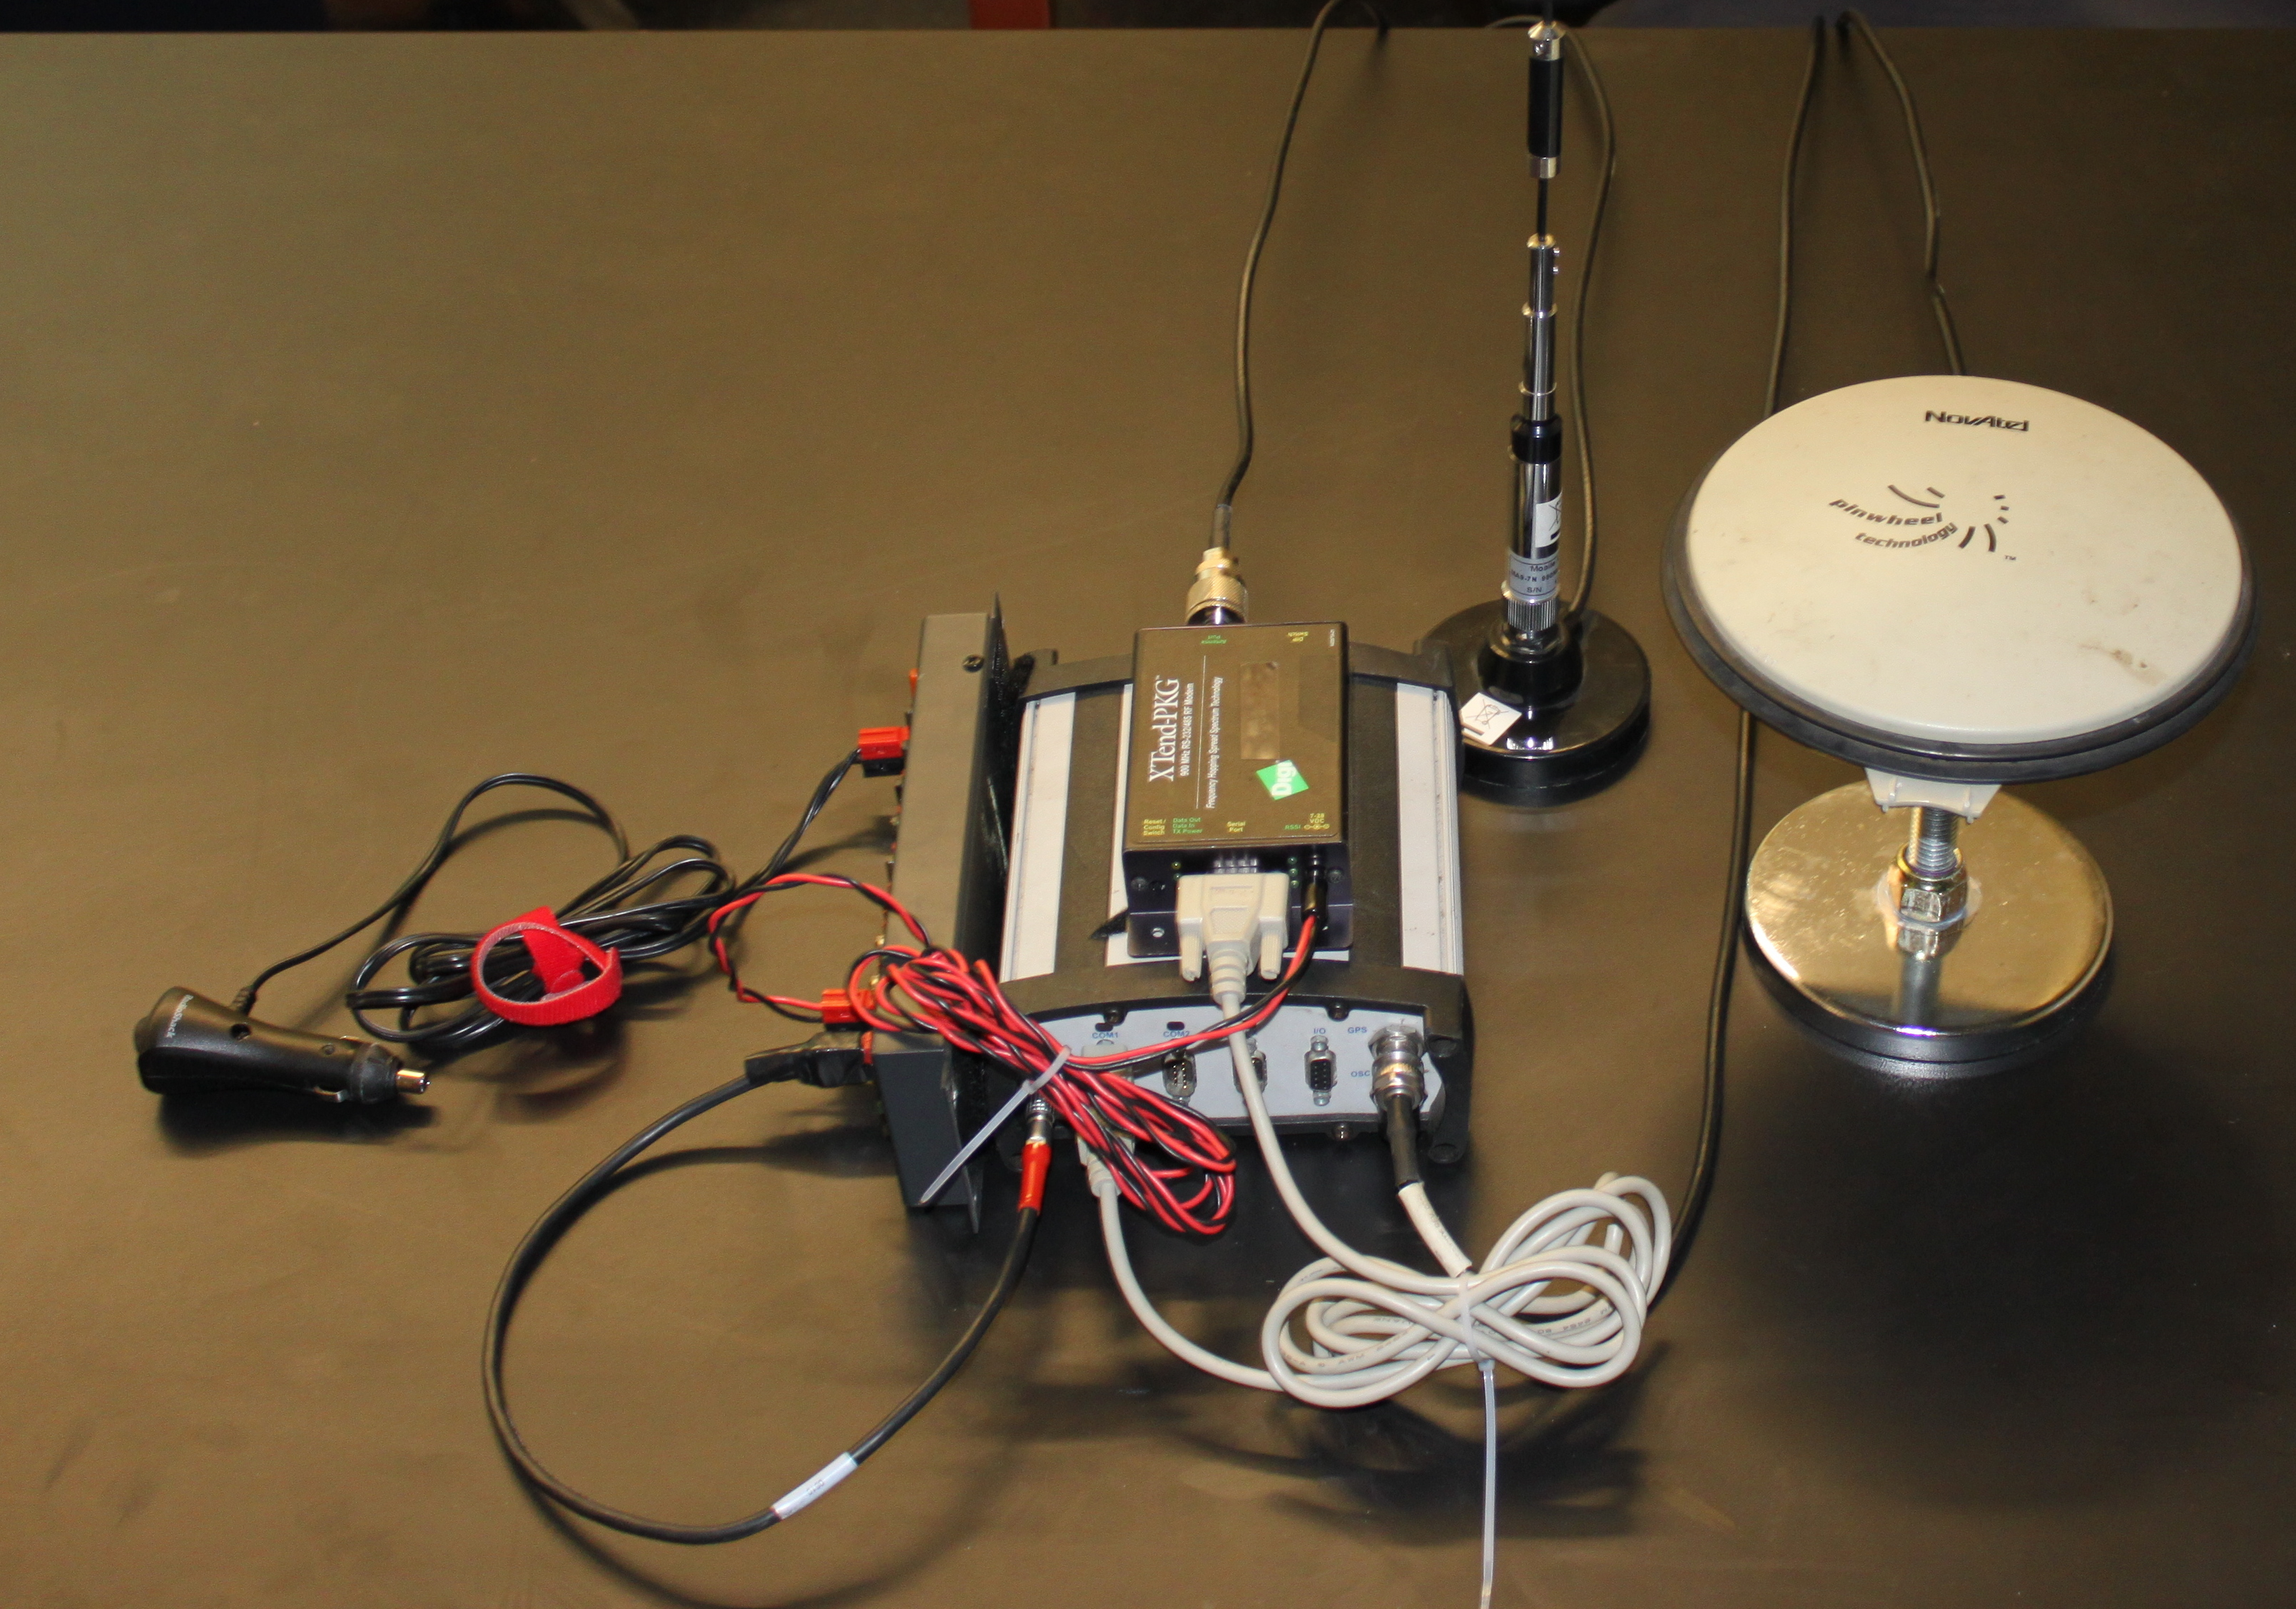
\includegraphics[width=\textwidth]{./figs/lead_hardware.jpg}
        \caption{Equipment used in the leading vehicle} \label{fig:hardwarelead}
    \end{minipage}
    \hspace{0.5cm}
    \begin{minipage}[b]{0.45\linewidth} \centering
        \includegraphics[width=\textwidth]{./figs/foll_antennae.jpg} 
        \caption{Antennaes as placed on either vehicle} \label{fig:antennaefoll}
    \end{minipage}
\end{figure}




%%%%%%%%%%%%%%%%%%%%%%%%%%%%%%%%%%%%%%%%%%%%%%%%%%%%%%%%%%%%%%%%%%%%%%%%%%%%%%%%
% What tests were performed
\section{Definition of Testing Procedures} \label{sec:test}

In order to formally quantify the ability of the tools developed in Chap. \ref{chap:gui} to assist convoy drivers in the target circumstances, three tests were devised: a lane change replication test, a target spacing maintenance test, and a limited visibility test. These were also conducted to compare and contrast the two approaches embodied by each GUI. 

\begin{figure}[ht] \centering
    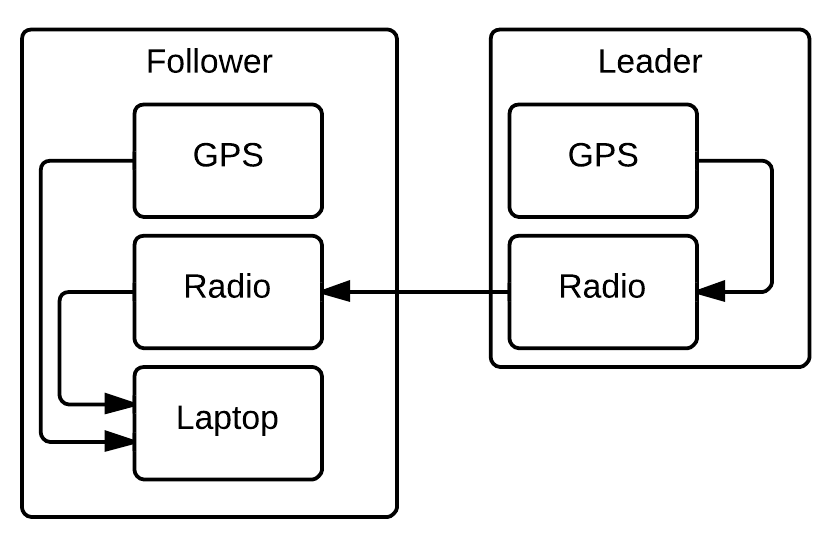
\includegraphics[width=4in]{./figs/hardware_flow.png}
    \caption{Flow of GPS data between leader and follower} \label{fig:hardwareflow}
\end{figure}

% data collection
Data collection can become an extremely memory intensive process, so selectivity was needed in choosing what data to record during testing. The stream of available data may be divided into two categories: raw GPS measurements which must be processed---the data flow for raw GPS measurements through hardware components is illustrated in Fig.~\ref{fig:hardwareflow}---and  data which is output to the GUI backend. During the develop-test-refine cycle, raw GPS measurements alone were recorded and then replayed to simulate online operation during algorithm tuning. However, when conducting experimental trials for formal analysis, only data streams which are consumed by the GUI are recorded in order to capture exactly what was displayed to the following driver and examine their resultant performance. Raw GPS measurements were excluded in order to reduce the volume of data throughput and increase computing efficiency.


%%%% Lane change replication
\subsection{Lane Change Replication Test} \label{sec:lanechangetest}
In determining the usefulness of any tool, it is highly desirable to devise a test which yields concise results, i.e., either pass or fail. To this end, a maneuver common in typical roadway driving, the lane change, was used in a situation in which the maneuver could be replicated properly or improperly to produce a binary result. This test takes place on the National Center for Asphalt Technology (NCAT) test track in Opelika, AL, which is a two lane, 1.7 mile oval oval with turns comparable to those found on an interstate highway. The leader drives through a $180^\circ$ turn and upon exiting makes a lane change between any of six cones spaced $10m$ apart along the center stripe at the start of the straightaway, as shown in Fig.~\ref{fig:lanechangediagram}. This event is visually obscured from the following driver, who has no foreknowledge of which cone pair will be chosen, so there is a $20\%$ chance of choosing the correct pair simply by guessing. This iteration of this test was performed twice, once with the monolithic GUI and once with the Earth-based GUI. No control run is needed, since a cumulative success rate across all iterations above $20\%$ represents an improvement from driving without navigation assistance. A range of highway driving speeds from 30 mph to 55 mph was used, and forward spacing was not examined except to ensure that it was large enough for the aforementioned visual obstruction.

\begin{figure}[ht] \centering
    \documentclass[10pt]{article}
\usepackage[utf8]{inputenc}
\usepackage{pgf,tikz}
\usetikzlibrary{arrows}
\pagestyle{empty}
\begin{document}
\definecolor{qqzzqq}{rgb}{0,0.6,0}
\definecolor{ttzzqq}{rgb}{0.2,0.6,0}
\definecolor{qqqqcc}{rgb}{0,0,0.8}
\definecolor{xdxdff}{rgb}{0.49,0.49,1}
\definecolor{ffcctt}{rgb}{1,0.8,0.2}
\definecolor{ffzzqq}{rgb}{1,0.6,0}
\definecolor{qqqqff}{rgb}{0,0,1}
\definecolor{cqcqcq}{rgb}{0.75,0.75,0.75}
\begin{tikzpicture}[line cap=round,line join=round,>=triangle 45,x=1.0cm,y=1.0cm]
\draw [color=cqcqcq,dash pattern=on 2pt off 2pt, xstep=2.0cm,ystep=2.0cm] (-0.94,-2.5) grid (29.18,16.12);
\draw[->,color=black] (-0.94,0) -- (29.18,0);
\foreach \x in {,2,4,6,8,10,12,14,16,18,20,22,24,26,28}
\draw[shift={(\x,0)},color=black] (0pt,2pt) -- (0pt,-2pt) node[below] {\footnotesize $\x$};
\draw[->,color=black] (0,-2.5) -- (0,16.12);
\foreach \y in {-2,2,4,6,8,10,12,14,16}
\draw[shift={(0,\y)},color=black] (2pt,0pt) -- (-2pt,0pt) node[left] {\footnotesize $\y$};
\draw[color=black] (0pt,-10pt) node[right] {\footnotesize $0$};
\clip(-0.94,-2.5) rectangle (29.18,16.12);
\draw [line width=5.2pt] (16,10)-- (2,10);
\draw [line width=5.2pt] (16,14)-- (2,14);
\draw [line width=5.2pt] (14,6)-- (16,6);
\draw [shift={(16,8)},line width=4.4pt,dash pattern=on 5pt off 5pt,color=ffcctt]  plot[domain=-1.57:1.57,variable=\t]({1*4*cos(\t r)+0*4*sin(\t r)},{0*4*cos(\t r)+1*4*sin(\t r)});
\draw [shift={(16,8)},line width=5.2pt]  plot[domain=-1.57:1.57,variable=\t]({1*6*cos(\t r)+0*6*sin(\t r)},{0*6*cos(\t r)+1*6*sin(\t r)});
\draw [shift={(16,8)},line width=5.2pt]  plot[domain=-1.57:1.57,variable=\t]({1*2*cos(\t r)+0*2*sin(\t r)},{0*2*cos(\t r)+1*2*sin(\t r)});
\draw [line width=4.4pt,dash pattern=on 5pt off 5pt,color=ffcctt] (14,4)-- (16,4);
\draw [line width=5.2pt] (16,2)-- (14,2);
\draw [line width=4.4pt,dash pattern=on 5pt off 5pt,color=ffcctt] (16,12)-- (4,12);
\draw [shift={(13.19,10.74)},line width=1.6pt,dotted,color=qqqqcc]  plot[domain=1.61:2.63,variable=\t]({1*2.58*cos(\t r)+0*2.58*sin(\t r)},{0*2.58*cos(\t r)+1*2.58*sin(\t r)});
\draw [shift={(8.37,13.37)},line width=1.6pt,dotted,color=qqqqcc]  plot[domain=4.97:5.79,variable=\t]({1*2.91*cos(\t r)+0*2.91*sin(\t r)},{0*2.91*cos(\t r)+1*2.91*sin(\t r)});
\draw [line width=1.6pt,dotted,color=qqqqcc] (13.08,13.32)-- (16.04,13.24);
\draw [shift={(16,8.05)},line width=1.6pt,dotted,color=qqqqcc]  plot[domain=-1.58:1.56,variable=\t]({1*5.19*cos(\t r)+0*5.19*sin(\t r)},{0*5.19*cos(\t r)+1*5.19*sin(\t r)});
\begin{scriptsize}
\fill [color=qqqqff] (16,6) circle (1.5pt);
\fill [color=qqqqff] (16,10) circle (1.5pt);
\fill [color=qqqqff] (16,2) circle (1.5pt);
\fill [color=qqqqff] (16,14) circle (1.5pt);
\fill [color=qqqqff] (2,10) circle (1.5pt);
\fill [color=qqqqff] (2,14) circle (1.5pt);
\fill [color=qqqqff] (14,6) circle (1.5pt);
\fill [color=ffzzqq] (4,12) circle (3.0pt);
\fill [color=ffzzqq] (6,12) circle (3.0pt);
\fill [color=ffzzqq] (8,12) circle (3.0pt);
\fill [color=ffzzqq] (10,12) circle (3.0pt);
\fill [color=ffzzqq] (12,12) circle (3.0pt);
\fill [color=ffzzqq] (14,12) circle (3.0pt);
\fill [color=qqqqff] (16,12) circle (1.5pt);
\fill [color=qqqqff] (16,4) circle (1.5pt);
\fill [color=qqqqff] (14,4) circle (1.5pt);
\fill [color=qqqqff] (14,2) circle (1.5pt);
\fill [color=qqqqff] (13.08,13.32) circle (1.5pt);
\draw[color=qqqqff] (13.24,13.58) node {$E$};
\fill [color=qqqqff] (11.56,12.74) circle (1.5pt);
\draw[color=qqqqff] (11.66,13) node {$J$};
\fill [color=xdxdff] (10.94,12) circle (1.5pt);
\draw[color=xdxdff] (11.1,12.26) node {$R$};
\fill [color=qqqqff] (10.14,11.06) circle (1.5pt);
\draw[color=qqqqff] (10.3,11.32) node {$U$};
\fill [color=ttzzqq,shift={(9.12,10.56)},rotate=90] (0,0) ++(0 pt,6.75pt) -- ++(5.85pt,-10.125pt)--++(-11.69pt,0 pt) -- ++(5.85pt,10.125pt);
\draw[color=ttzzqq] (8.86,11.02) node {$Leader$};
\fill [color=qqqqff] (16.04,13.24) circle (1.5pt);
\draw[color=qqqqff] (16.22,13.5) node {$W$};
\fill [color=qqzzqq,shift={(15.96,2.86)},rotate=270] (0,0) ++(0 pt,6.75pt) -- ++(5.85pt,-10.125pt)--++(-11.69pt,0 pt) -- ++(5.85pt,10.125pt);
\draw[color=qqzzqq] (15.32,3.32) node {$Follower$};
\end{scriptsize}
\end{tikzpicture}
\end{document}
    \caption{Diagram of the lane change replication test procedure} \label{fig:lanechangediagram}
\end{figure}

The lane change replication test focused on aiding a driver in conditions where visibility is totally denied, as foliage and terrain features lie between the two vehicle during the moment of interest. Sensor and display frequencies will play a large role in this outcome. If information is updated with real time interpolation, a delay of at least one timestep (not including calculation time) is present, meaning that a worst-case GPS output frequency of 1.0 Hz will result 1.0 s data lag. When this is the case, the error in . The impact of that behavior is one thing being examined in the lane change replication test. For the monolithic GUI, this test will show whether the range scaling indicators adequately convey distance information so that a driver can determine where to turn, when the interpolation functionality is disabled for rapid updating. Sec. \ref{sec:lanechangetestresults} outlines the results of the lane change replication test.

%%%% Target Spacing Test
\subsection{Precision Following Test} \label{sec:targetspacingtest}
The lane change replication test is one example of implementing the path duplication tool, but does not produce the detailed results necessary for a formal conclusion favoring the usefulness of one GUI over the other. Centimeter-level measurements are available, so it is of great interest to determine whether either tool enables a convoy driver to carry out the following task with this improved level of precision. The precision following test begins and ends with both vehicles parked atop the center stripe of the NCAT test track. The lead vehicle accelerates to approximately 45 mph then begins a sinusoidal path with a mean about the center stripe, a period of approximately 10 s, and an amplitude that puts the wheels of the lead vehicle upon the outermost lane marking at the peaks. Once reaching 45 mph, the magnitude of the leader's ground plane velocity vector will vary according to position on the track. Along the two 180$^\circ$ turns it will be approximately 45 mph, and along the straightaways it will be approximately 65 mph. Throughout the test, the following driver is attempting to maintain a inter-vehicular spacing as low as possible without incurring any distance alerts, and accumulate as little deviation over time as possible.

% % \documentclass[10pt]{article}
% \usepackage[utf8]{inputenc}
% \usepackage{pgf,tikz}
% \usetikzlibrary{arrows}
% \pagestyle{empty}
% \begin{document}

%<<<<<<<WARNING>>>>>>>
% PGF/Tikz doesn't support the following mathematical functions:
% tan, cosh, acosh, sinh, asinh, tanh, atanh

% Plotting will be done using GNUPLOT
% GNUPLOT must be installed and you must allow Latex to call external programs by
% Adding the following option to your compiler
% shell-escape    OR    enable-write18 
% Example: pdflatex --shell-escape file.tex 

    
    \definecolor{qqttff}{rgb}{0,0.2,1}
    \definecolor{ffccqq}{rgb}{1,0.8,0}
    \begin{tikzpicture}[line cap=round,line join=round,>=triangle 45,x=1.0cm,y=1.0cm, scale=0.6]
        \clip(-2.3,-1.64) rectangle (27.4,16.98);
        \draw [line width=4.4pt] (0,4)-- (20,4);
        \draw [line width=4.4pt] (0,0)-- (20,0);
        \draw [line width=2.4pt,dash pattern=on 5pt off 5pt,color=ffccqq] (0,2)-- (20,2);
        \draw[line width=2pt,dotted,color=qqttff, smooth,samples=100,domain=0.0:20.0] plot[parametric] function{t,1.5*sin((t/2)*180/pi)+2};
        \draw (3.38,4)-- (3.38,4.5);
        \draw (15.88,4.5)-- (15.88,4);
        \draw [->] (3.55,4.25) -- (15.7,4.25);
        \begin{scriptsize}
            \draw[color=black] (10.14,4.46) node {T = 10 s};
        \end{scriptsize}
    \end{tikzpicture}


% \end{document}
\begin{figure}[ht] \centering
    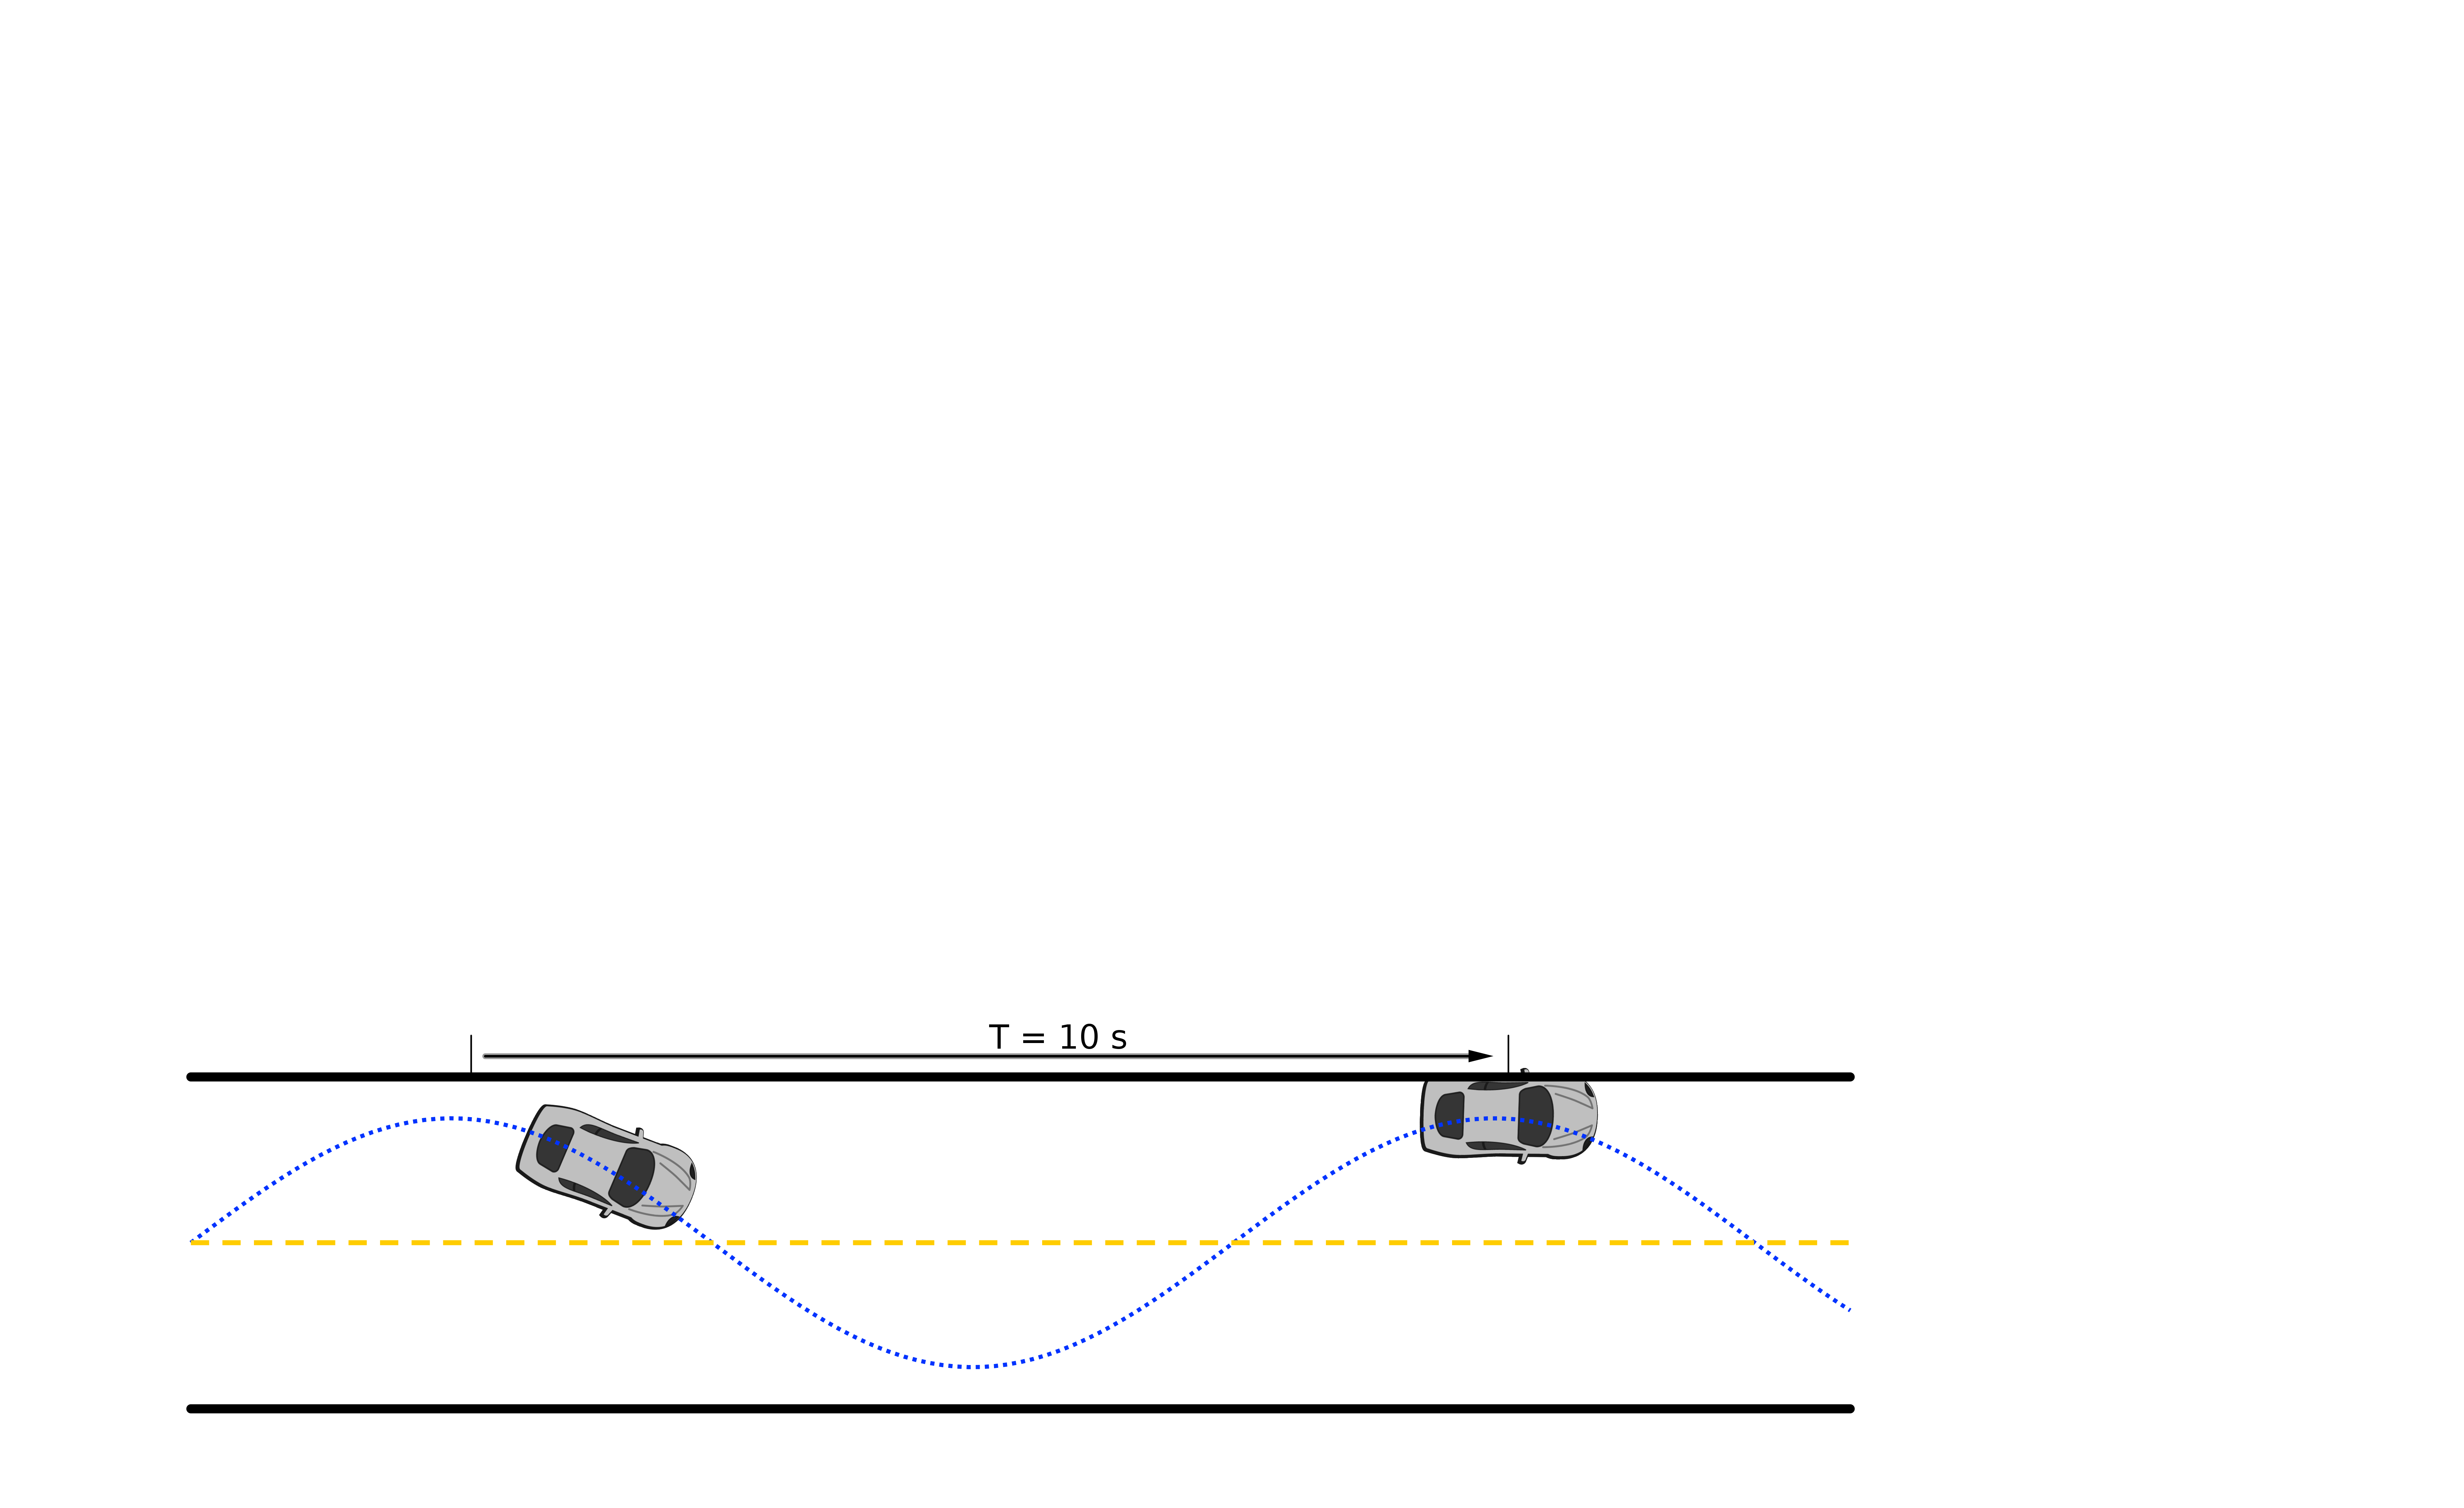
\includegraphics[width=6.5in]{./figs/precision_following_diagram.png}
    \caption{Diagram of the precision following test procedure} \label{fig:precisionfollowingdiagram}
\end{figure}

This test primarily focused on distinguishing which GUI best provided aid in path duplication; for a comparative analysis, the test was conducted with the aid of each GUI individually, then without any assistance information at all. As this test was conducted in an environment equivalent to most American two-lane roads and the leader does not stray from the two outer lane markings, it was anticipated that the lateral deviation should be bounded by approximately the width of the road minus the track width of the widest vehicle, or $5.8~m$. This allows for scrutiny of the deviation in greater detail than when the lateral deviation is not bounded by design. Sec. \ref{sec:precisionfollowingresults} outlines the results of the precision following test.

\subsection{Zero Landmark Test} \label{sec:zerolandmarktest}
The precision following test took place in an environment abundant in visual landmarks by which to localize, such as lane markings and road signs. Given the motivation for these tools, it is necessary to examine the performance of both GUIs in a situation where this type of assistance is denied. The zero landmark test was therefore constructed to determine the impact of removing visual awareness of surrounds as well as waypoints along the leaders path to assist in replicating it.

Both vehicles began parked in a large, open expanse of flat asphalt (`skidpad') with excellent GPS coverage. There are no clearly visible artifacts upon the ground, though some objects are visible at the outer edges of the skidpad. To further obscure visual following, the test was conducted at night. The lead vehicle drove in chaotic patterns intended present a path with is difficult to follow while the following vehicle attempted to adhere to the path as well as possible and maintain the closest possible curvilinear separation distance without triggering any alert messages. Sec. \ref{sec:zerolandmarkresults} outlines the results of the zero landmark test, and the path taken by the leader in one of the runs is shown in Fig.~\ref{fig:zerolandmarkpath}

\begin{figure}[ht] \centering
    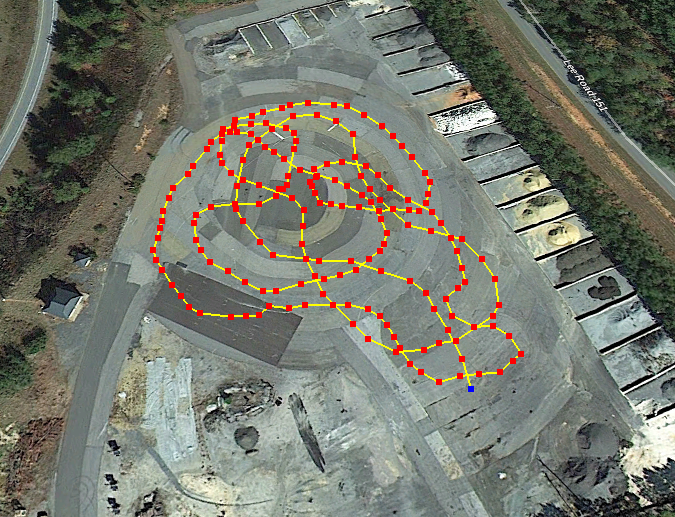
\includegraphics[width=5in]{./figs/zero_landmark_path.png}
    \caption{Path taken by lead vehicle during a single run of the zero landmark test} \label{fig:zerolandmarkpath}
\end{figure}






%%%%%%%%%%%%%%%%%%%%%%%%%%%%%%%%%%%%%%%%%%%%%%%%%%%%%%%%%%%%%%%%%%%%%%%%%%%%%%%%
% Results section
\section{Results} \label{sec:results}

In processing the collected data, some
% technicalities
When at any point a path is uncalculable, due to satellite outage, outlying values, course errors, or other errors, the path reported is of length one (a single point at the position of the leader). When this occurs, the following distance becomes 0.0, and these instances were ignored in tabulation of the following distance score.


%%%%% Lane Change between Cones
\subsection{Lane Change Replication Test Results} \label{sec:lanechangetestresults}

Table \ref{tab:lanechangeresults} shows the results of all runs of the lane change replication test. It is plain to see that in every instance where a lane change was made between the improper cone pair, the follower changed lanes later than did the leader. This is attributed to latency existing in the combined system from calculation and driver reaction.

\begin{table}[htbp] \centering \caption{Cone pairs chosen in the lane change replication test}
\begin{tabular}{c|cc} 
    Run \#  &     Leader&    Follower \\ \hline\hline
    1       &       1   &    3 \\
    2       &       3   &    4   \\
    3       &       2   &    3   \\
    4       &       5   &    5 \\ \hline   
\end{tabular} \label{tab:lanechangeresults} \end{table}

Figures~\ref{fig:lanechange_earth} and~\ref{fig:lanechange_mono} show what the driver saw onscreen prior to attempting to make the correct lane change using the Earth GUI and the monolithic GUI, respectivley.

\begin{figure}[ht] \centering
    \begin{minipage}[b]{0.45\linewidth} \centering 
        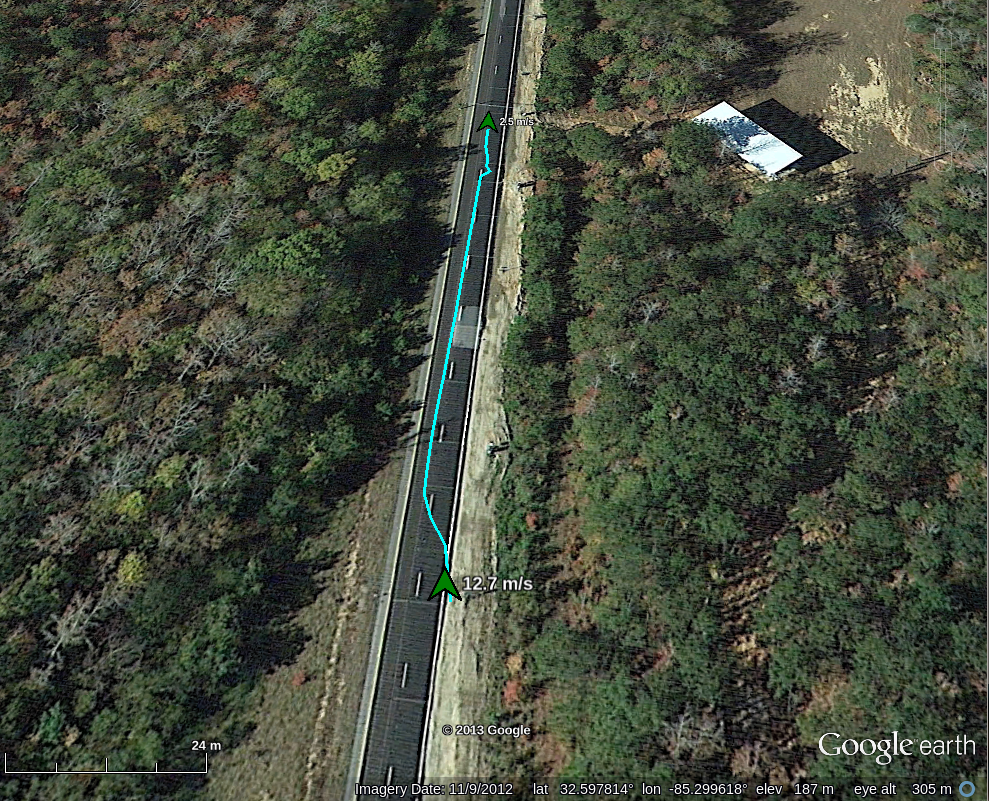
\includegraphics[width=3in]{./figs/lane_change.png}
        \caption{Earth GUI as follower enters a lane change} \label{fig:lanechange_earth}
    \end{minipage}
    \hspace{0.5cm}
    \begin{minipage}[b]{0.45\linewidth} \centering
        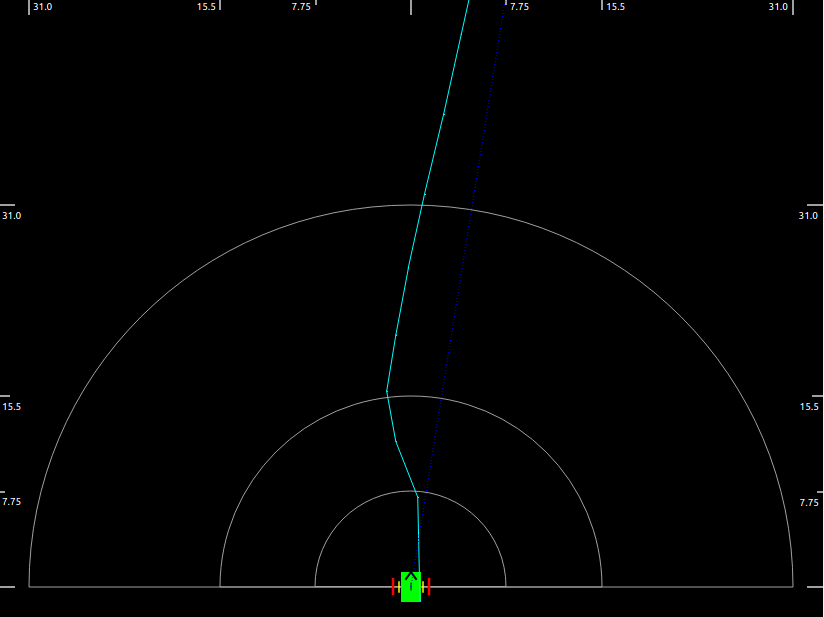
\includegraphics[width=3in]{./figs/lane_change_mono.png}
        \caption{Monolithic GUI as follower enters a lane change} \label{fig:lanechange_mono}
    \end{minipage}
\end{figure}





%%%%% Follow the Path around the track
\subsection{Precision Following Test Results} \label{sec:precisionfollowingresults}

% Explain the run-specific charts
Shown in Figs. \ref{fig:precisionresults_earth} , \ref{fig:precisionresults_monolith} , and \ref{fig:precisionresults_control} are the best of all runs of the precision following test using the Earth-based GUI, monolithic GUI, and no GUI at all, respectivley. The criterion for selecting the `best' run was that which had the lowest combined percentage of timesteps when an alert was issued for either distance or deviation. Figure \ref{fig:precision_alerts} outlines how often alerts occurred during each data run.





%%%%% Skidpad drive around
\subsection{Zero Landmark Test Results} \label{sec:zerolandmarkresults}

% Explain the run-specific charts
Shown in Figs. \ref{fig:zeroresults_earth} , \ref{fig:zeroresults_monolith} , and \ref{fig:zeroresults_control} are the best of all runs of the zero landmark test using the Earth-based GUI, monolithic GUI, and no GUI at all, respectivley. The criterion for selecting the `best' run was that which had the lowest combined percentage of timesteps when an alert was issued for either distance or deviation. Figure \ref{fig:zero_alerts} outlines how often alerts occurred during each data run.

